%%
% SigLog paper on HoTT
% May 2014
% IHP
%%
\documentclass[11pt]{article}
\usepackage{amsmath}
\usepackage{amssymb,latexsym}
\usepackage{amsthm}
\usepackage{bm}
\input{prooftree}
\usepackage[all,cmtip]{xy}
\input{diagxy}
\CompileMatrices       
\usepackage{url}
\usepackage{tikz}
\usepackage{pdfpages}

\usepackage[color=green!40]{todonotes}



% categories
\newcommand{\C}{\ensuremath{\mathbb{C}}}
\newcommand{\B}{\ensuremath{\mathbb{B}}}
\newcommand{\N}{\ensuremath{\mathbb{N}}}
\newcommand{\T}{\ensuremath{\mathbb{T}}}
\newcommand{\CC}{\ensuremath{\mathcal{C}}}
\newcommand{\BB}{\ensuremath{\mathcal{B}}}
%\newcommand{\EE}{\ensuremath{\mathcal{E}}}
\newcommand{\psh}[1]{\ensuremath{\mathsf{Set}^{#1^{\mathrm{op}}}}}
\newcommand{\Set}{\ensuremath{\mathsf{Set}}}
\newcommand{\Cat}{\ensuremath{\mathsf{Cat}}}
\newcommand{\covpsh}[1]{\ensuremath{\mathsf{Set}^{#1}}}
%\renewcommand{\to}{\ensuremath{\rightarrow}}
\newcommand{\pocorner}[1][dr]{\save*!/#1+1.2pc/#1:(1,-1)@^{|-}\restore}
\newcommand{\pbcorner}[1][dr]{\save*!/#1-1.2pc/#1:(-1,1)@^{|-}\restore}
\newcommand{\y}{\ensuremath{\mathsf{y}}} % Yoneda embedding

% arrows
\newcommand{\hook}{\ensuremath{\hookrightarrow}}
\newcommand{\mono}{\ensuremath{\rightarrowtail}}
%\newcommand{\epi}{\ensuremath{\twoheadrightarrow}}


% cubical sets
\newcommand{\I}{\ensuremath{\mathrm{I}}}
\renewcommand{\H}{\ensuremath{\mathbb{H}}}
\newcommand{\HH}{\ensuremath{\mathcal{H}}}

% type theory
\newcommand{\G}{\ensuremath{\Gamma}}
\newcommand{\defeq}{=_{\mathrm{def}}}
\newcommand{\type}{\mathsf{type}}       
\newcommand{\types}[2]{#1 \vdash #2:\type}
\newcommand{\Gtypes}[1]{\types{\Gamma}{#1}}
\newcommand{\term}[2]{#1\,:\,#2}
\newcommand{\terms}[2]{#1 \vdash #2}
\newcommand{\Gterms}[1]{\terms{\Gamma}{#1}}
\newcommand{\ext}[2]{{#1\!\centerdot\! #2}}
\newcommand{\ty}{\ensuremath{\,:\,}}
\newcommand{\pair}[1]{\ensuremath{\langle #1\rangle}}
\newcommand{\exdot}{\ensuremath{\!\centerdot\!}}
\newcommand{\texdot}{\ensuremath{\centerdot}}

% Id types
\newcommand{\Id}{\mathsf{Id}}
\newcommand{\id}[1]{\Id_{#1}}
\newcommand{\refl}{\mathsf{refl}}
\newcommand{\rec}{\mathsf{rec}}
\newcommand{\idrec}{\mathsf{idrec}}
\newcommand{\jay}{\mathsf{j}}
\renewcommand{\i}{\mathsf{i}}

% Universe
\newcommand{\U}{\ensuremath{\mathcal{U}}}
\newcommand{\UU}{\ensuremath{\widetilde{\mathcal{U}}}}

% theorem styles
\newtheorem{theorem}{Theorem}
\newtheorem*{theorem*}{Theorem}
\newtheorem{proposition}[theorem]{Proposition} 
\newtheorem{lemma}[theorem]{Lemma}
\newtheorem{corollary}[theorem]{Corollary} 

\theoremstyle{remark}
\newtheorem{remark}[theorem]{Remark} 
\newtheorem*{remarks*}{Remarks}
\newtheorem{example}[theorem]{Example}

\theoremstyle{definition}
\newtheorem{definition}[theorem]{Definition}

%%%%%%%%%%%%%%%%%%%%%%%%%%%%%%%%%%%%%%%%%%%%%%%%%%%%
\begin{document}
%%%%%%%%%%%%%%%%%%%%%%%%%%%%%%%%%%%%%%%%%%%%%%%%%%%%

\title{Homotopy Type Theory and Univalent Foundations}
\author{Steve Awodey \and Robert Harper}
\date{\today}

\maketitle
%%%%%%%%%%%%%%%%%%%%%%%%%%%%%%%%%%%%%%%%%%%%%%%%%%%%

Homotopy Type Theory is an emerging unification of previously disparate frameworks for formalizing and mechanizing
mathematics, one based on a computational conception of the type of a construction, the other based on a homotopical
conception of the (homotopy) type of a space.  Indeed, the name ``homotopy type theory'' can be read in two ways, as
``(homotopy type) theory'' and ``homotopy (type theory)'', neatly summarizing the consolidation of ideas at the heart of
the subject.  The computational notion of type has its origins in Brouwer's program of intuitionism, which sought to
ground mathematics in the concept of an effective construction (one would say ``algorithm'' these days).  The
homotopical notion of type emerges from abstract homotopy theory, in particular Grothendieck's conception of a space as
an $\infty$-groupoid.  The computational perspective was developed most fully by Per Martin-L\"{o}f, leading in
particular to his Intuitionistic Theory of Types~\cite{mltt}, on which the formal system of homotopy type theory is
based.  The connection to homotopy theory was first hinted at in the groupoid interpretation of Hofmann and
Streicher~\cite{HS} and then made explicit by Awodey and his students Lumsdaine and Warren~\cite{AW,AL}, who showed that
every type in Martin-L\"{o}f's system has the structure of an $\infty$-groupoid, and that the entire system can be
interpreted in any Quillen model category, an abstract framework for doing homotopy theory.  The connection was clinched
by Voevodsky's introduction of the \emph{univalence axiom}, which is motivated by the homotopical interpretation, which
relates type equality to homotopy equivalence.

Because univalence plays such a central role, Voevodsky has suggested that the unification of the computational and
homotopical perspectives be called the \emph{Univalent Unification}\todo[author=RH]{citation required, maybe ias
  article?} of two major lines of development in mathematics.  A critically important point is that the univalent
unification is \emph{fully compatible} with classical mathematics; it does not involve any principles that are
incompatible with classical reasoning, though it does, at the outset, avoid postulating axioms that are unnecessary for
much of the development.  Indeed, the formal system of homotopy type theory contains within it the whole of ZF set
theory, with or without the Axiom of Choice, and with or without the Law of the Excluded Middle, two principles that lie
at the heart of classical mathematics and that have, regrettably, been obstacles to the kind of unification described
here.  By not insisting on these axioms globally, it is possible to consider a far richer notion of type than has
hitherto been possible in the computational setting, namely one in which types are abstract spaces that can have
non-trivial higher-dimensional structure, as exemplified by familiar examples such as the $n$-spheres for all $n\geq 0$.
Rather than being ``coded up'' as certain structured sets representing certain conceptions of space, such as a
topological space, these objects instead arise \emph{synthetically} within the theory.  They are characterized by their
introductory and eliminatory forms (mapping-in and mapping-out properties, or universal properties), rather than by how
they are constructed as sets.  This perspective greatly simplifies many familiar constructions in homotopy theory, such
as homotopy groups~\cite{LS-Circ}, truncations~\cite{truncations}, and Eilenberg-MacLane spaces~\cite{LF-EM}, and
supports remarkably simple and clear proofs of well-known results, such as calculations of the higher homotopy groups of
the spheres~\cite{LB-PinSn}.  In this way it is possible to unify standard, classical logic and set theory with
constructive logic and type theory by regarding the former as the logic of a very special kind of objects (namely,
sets), and the latter as the general logic that applies not only to sets (the $0$-level spaces), but also to higher
types of spaces.

What is it that makes the univalent unification possible?  Although it may be too early to formulate a single, deep
unifying principle, it is possible to make a few observations that will give the reader a sense of its inevitability.
First, all of the constructions of Intuitionistic Type Theory, including especially the previously enigmatic identity
type, are homotopy invariant, in the both sense that type families and mappings between types inherently respect
``paths'' in spaces, representing \emph{identifications} of points in the space, and that the formation of type-indexed
products and sums of types, which correspond to analogous constructions on spaces, respect the homotopically motivated
notion of type equivelence.  This invariance essentially follows from the basic fact that Martin-L\"{o}f's identity
type, taken as a whole, corresponds to the \emph{total path space} of a space (see \cite{AW}); since everything in the
formal system respects identity, everything in the interpretation respects homotopy, which is determined by
identfication along paths.  Second, a characteristic feature of both intuitionistic type theory and higher homotopy
theory is the emphasis on \emph{structure} over \emph{property}.  In intuitionistic mathematics types express
propositions, and objects of the type are proofs of those propositions in the form of mathematical constructions that
provide evidence for their truth.  A similar emphasis is found in abstract homotopy theory, in which paths (homotopies)
may be seen as evidence for the identification (in a sense, ``equality'') of two points, and similarly for paths between
the corresponding values of two functions.  Two points are not merely equal as a property, but rather are identified by
a (not necessarily unique) construction.  This approach extends to higher dimensions in that one may speak of the
identification of two (parallel) identifications, at all higher dimensions.  Such a structure of a hierarchy of
identifications via path connectedness is found in standard settings for homotopy theory such as simplicial sets,
cubical sets, and globular sets, all of which stress the role of cells as identifications.

The hierarchy of possible identifications leads to Voevodsky's conception of a hierarchy of homotopy levels, or h-levels
for short, definable within type theory.  Whereas the usual hierarchy of size is determined by type universes or large
cardinals in type theory or set theory, the hierarchy of h-levels is based not on the size, but on the internal
structure of a type.  Roughly speaking, the lowest level consists of the types that have at most one element, called
\emph{propositions}.  The next level, called \emph{sets}, consists of those whose identity types are propositions. After
that come the types whose identity types are sets: the \emph{groupoids}.  And so on.  Just the recognition that this
hierarchy of h-levels is present in the system of all types has been a huge advance in our understanding of type theory;
previously, it was simply a mystery that some types were fully determined by their elements, while others seemed to
behave as though they had some further structure.  The construction of quotient types, for example, is now greatly
simplified when one knows that the equivalence relation being factored out is a family of propositions, and not
``higher" types.  For another example, for types $A$ and $B$ that are propositions, the relevant notion of equivalence
is \emph{logical equivalence}, represented by the type $A\leftrightarrow B$.  For sets, the relevant notion is
\emph{isomorphism} $A\cong B$, and for groupoids, there is the notion of \emph{(categorical) equivalence} $A\simeq B$.
Each of these concepts results by specializing the single, uniform notion of \emph{equivalence of types} $A\simeq B$ to
the respective cases of propositions, sets, and groupoids.  In this setting, the new univalence axiom can be stated as
the assertion that the type $A\simeq B$ of all equivalences between two types $A$ and $B$ is itself equivalent to their
identity type,
\[\tag{UA}
(A\simeq B)\ \simeq\  \id{}(A,B).
\]
Thus in particular, logically equivalent propositions will be identified, as in the original, extensional type theory of
Church \cite{Church}.  Isomorphic sets, too, will be identified ``up to homotopy'', \textit{i.e.}\ by paths between them in the
universe of all types, and similarly for equivalent groupoids, and equivalent types in general.

This is not really the place for a systematic introduction (for that, see \cite{HoTTbook}), or even a general survey
(such as \cite{apw,pw}), but a brief example may serve to convey a bit of the flavor of the new approach, especially the
distinctive intermingling of logical and homotopical ideas.  As is the case in conventional Martin-L\"of type theory,
the basic types of booleans $\B$ and natural numbers $\N$ can have at most one identification between any two elements;
that is, given say $n, m : \N$ and $p,q: \id{\N}(n,m)$ in the identity type of $n$ and $m$, we always have
$\alpha:\id{\left(\id{\N}(n,m)\right)}(p,q)$ identifying $p$ and $q$.  In this sense, there is no real information in
the type $\id{\N}(n,m)$, apart from whether or not it is inhabited.  Such types with at most one identification between
any two elements are called (``homotopy 0-types'' or simply) ``sets''.  Any types that can be constructed from $\B$,
$\N$, or any other sets, by means of the usual type constructors of dependent sum $(\Sigma{x:A})B(x)$ and dependent
product $(\Pi{x:A})B(x)$ (which includes $A\times B$ and $A\rightarrow B$ as special cases) are also sets, and the same
is true for the equality types $\id{A}(a,a')$ for $a,a':A$, for any set $A$.

 An example of a type that is not a set is the circle (or ``$1$-sphere'') $S^1$, which has a base point $b: S^1$ with many different self-identifications $\refl(b),\, p,\, p\cdot p,\, ... :\id{S^1}(b,b)$.  Here $\refl(b)$ is the trivial identification, \textit{i.e.}\ the canonical witness to the reflexivity of identity, but there is also another identification $p$ which is different from $\refl(b)$ in the sense that $\id{\left(\id{S^1}(b,b)\right)}(\refl(b), p)$ is empty.  We can think of $p$ homotopically as the continuous ``path" that goes once around the circle. 

%
\missingfigure[figwidth=3in]{draw a circle here, with $b$ and $p$ indicated}
%

By the (function witnessing the) transitivity of equality, 
\[
(-)\cdot(-) : \id{S^1}(a,b) \times \id{S^1}(b,c)\to \id{S^1}(a,c),
\]
 there are also the ``paths'' $p\cdot p,\, p\cdot p\cdot p,\, \ldots$.   And by symmetry,
 \[
 (-)^{-1}:\id{S^1}(a,b) \to \id{S^1}(b,a),
 \]
 there are similarly the paths $p^{-1},\, p^{-1}\cdot p^{-1}, \ldots :\id{S^1}(b,b)$.  Although $S^1$ is therefore not a set, it can be shown that $\id{S^1}(b,b)$ is one; that is, the types $\id{\left(\id{S^1}(b,b)\right)}(x,y)$ are either inhabited (by reflexivities) or empty, depending on whether or not $x=y$, for all $x,y : \id{S^1}(b,b)$ --- we say that $S^1$ is a ``(homotopy) 1-type".  This fact follows from the specification of $S^1$ as a new kind of \emph{higher} inductive type, generalizing the usual specification of the natural numbers and similar structures.  For $S^1$, the inductive specification essentially says that $S^1$ is the type freely generated by the base point $b:S^1$ and the loop $p:\id{S^1}(b,b)$, in the same sense that the usual inductive specification of $\N$ says that it is the type freely generated by $0:\N$ and the successor function $s:\N\to\N$.  
  
Another type that is not a set is the universe $\U$ of all (small) types.  According to the Univalence Axiom, identifications between types $A,B:\U$ correspond to equivalences $A\simeq B$, which are generalized type isomorphisms.  In fact, as already stated, if $A$ and $B$ themselves are sets, then an equivalence between them is just an isomorphism in the usual sense: a pair of maps back and forth that compose to the respective identity mapppings.  Now the booleans $\B$, for example, have two different isomorphisms $\B\simeq \B$, namely the identity and the operation of ``negation'' $\neg:\B\to\B$, which swaps the truth values $0,1:\B$.  Thus by univalence there are two distinct identifications in $\id{\U}(\B,\B)$, corresponding to these distinct isomorphisms, and so $\U$ is not a set, but, like $S^1$, a ``higher-dimensional" type.  
 
Now observe that by the basic recursive property of $S^1$ as ``the type freely generated by a point and a loop on it'', there is a map $$\rec(\B,n): S^1 \to \U$$ determined by sending the base point $b:S^1$ to the booleans $\B:\U$ and the generating loop $p : \id{S^1}(b,b)$ to (the loop corresponding under univalence to) negation, say $n : \id{\U}(\B,\B)$.  As a type of the form $\B\to\U$, this $\rec(\B,n)$ is thus a family of types over $\B$, sometimes called a ``dependent type" and written $x:\B \vdash \rec(\B,n)(x)$.  Homotopically, such a type-family is interpreted as a ``fibration" $E\to\B$, where the total space $E$ is just the sum type $(\Sigma{x:\B})\rec(\B,n)(x)$, equipped with its usual indexing projection.  In the present case, the ``fiber" is then the type $\rec(\B,n)(b) = \B$, and the action on (elements of) $\B$ induced by the path $n: \id{S^1}(b,b)$ in the base is exactly the operation of negation $\neg : \B\to \B$.  Thus, from a homotopical point of view, we have constructed the ``twisted double cover'' of the circle (see Figure \ref{fig:winding}).
%
\todo[inline]{fix this figure}
%
\begin{figure}\centering
  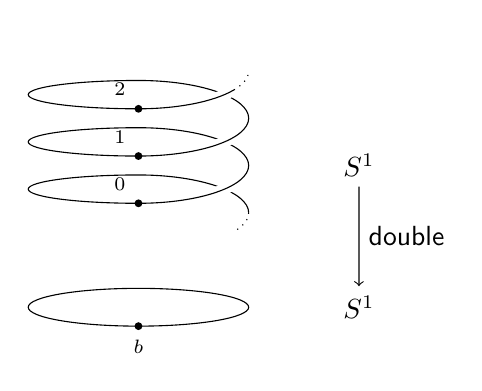
\begin{tikzpicture}[xscale=1.4,yscale=.6]
    \node (R) at (2,1) {$S^1$};
    \node (S1) at (2,-2) {$S^1$};
    \draw[->] (R) -- node[auto] {$\mathsf{double}$} (S1);
    \draw (0,-2) ellipse (1 and .4);
    \draw[dotted] (1,0) arc (0:-30:1 and .8);
    \draw (1,0) arc (0:90:1 and .8) arc (90:270:1 and .3) coordinate (t1);
    \draw[white,line width=4pt] (t1) arc (-90:90:1 and .8);
    \draw (t1) arc (-90:90:1 and .8) arc (90:270:1 and .3) coordinate (t2);
    \draw[white,line width=4pt] (t2) arc (-90:90:1 and .8);
    \draw (t2) arc (-90:90:1 and .8) arc (90:270:1 and .3) coordinate (t3);
    \draw[white,line width=4pt] (t3) arc (-90:90:1 and .8);
    \draw (t3) arc (-90:-30:1 and .8) coordinate (t4);
    \draw[dotted] (t4) arc (-30:0:1 and .8);
    \node[fill,circle,inner sep=1pt,label={below:\scriptsize $b$}] at (0,-2.4) {};
    \node[fill,circle,inner sep=1pt,label={above left:\scriptsize 0}] at (0,.2) {};
    \node[fill,circle,inner sep=1pt,label={above left:\scriptsize 1}] at (0,1.2) {};
    \node[fill,circle,inner sep=1pt,label={above left:\scriptsize 2}] at (0,2.2) {};
  \end{tikzpicture}
  \caption{The twisted double cover of $S^1$ in classical topology}\label{fig:winding}
\end{figure}
%
This important construction from homotopy theory is closely related to the celebrated Hopf fibration which, among other things, can be used to compute some of the higher homotopy groups of the spheres $S^2$ and $S^3$.  Indeed, one can construct the Hopf fibration in homotopy type theory in much the same way as the foregoing example, using univalence, negation, winding around the circle, and other constructions derived from combinations of logical, type-theoretic, and homotopical ideas.  This sort of reasoning gives an entirely new ``synthetic" approach to some areas of classical mathematics like algebraic topology, which not only allows for the explicit logical formalization of classical results like the calculations of homotopy groups of spheres, but also permits their formal verification in computational proof systems based on a constructive system of logic.

%%%%%%%%%%%%
%
% the following bit expands on some of the material in 107-129, but also conflicts with it in some places 
% (e.g. "n-type" vs. "h-level").
% I have tried below to revise to avoid some repetition and make it more consistent, but this is just a suggestion.
% I am leaving the original here in comments for comparison and possible reuse.
%
%%%%%%%%%%%%
%
%An important point about univalent foundations is that it subsumes the classical set-theoretic framework for doing
%mathematics.  The hierarchy of $n$-types neatly accounts for classical set-theoretic foundations within a broader
%framework of homotopy types.  Specifically, $-1$-types, which have at most one element up to higher identification,
%correspond to classical proof-irrelevant propositions, except that whether to insist that every proposition be inhabited
%or empty remains a consistent choice that one may accept or reject at will.  The $0$-types, for which equality is a
%classical proposition ($-1$-type) that is taken to be ``self-evident'' or ``proof-irrelevant'' correspond to classical
%sets, without prior commitment to choice principles or whether membership is a boolean proposition; these can be taken
%as axioms according to preference, without fear of inconsistency.  The advantage of univalent foundations is that
%besides the familiar concepts of proposition (classically formalized as predicate calculus) and set (classically given
%by the Zermelo-Fr\"{a}nkel axioms), it provides an infinite hierarchy of dimensions extending beyond just these two.
%For example, the $1$-types are the natural setting for set-theoretic structures, such as groups or rings, that one may
%wish to identify up to isomorphism.  Because two groups, say, can be isomorphic in different ways, the evidence for
%their identification must provide the mutually inverse pairs of homomorpisms that constitute the identification.
%
%Another import aspect of univalent foundations is that it extends Martin-L\"{o}f's type theory~\cite{mltt} with an
%infinite hierarchy of dimensions that were hitherto inaccessible within the theory, even though models were known that
%exhibited higher-dimensional structure~\cite{HS}.  Type theory was conceived as a foundation for
%constructive mathematics, in which all constructions, including proofs of propositions, have direct computational
%meaning in accordance with Brouwer's original program.  This connection with computation has proved enormously
%influential in computer science, in particular in the theory of programming languages and the foundations of mechanized
%proof.  At present homotopy type theory exploits the concept of proof relevance that is central to the constructivist
%program (indeed, according to that program propositions are not just $-1$-types, but can be any $n$-type), and draws on
%the emphasis on abstract types (for example, in the treatment of the identification type as an abstraction in itself,
%rather than being encoded in terms of a concrete conception of homotopy).  The grand challenge is to extend the
%computational interpretation to the full hierarchy of $n$-types, providing a computational meaning for, say, mappings
%among higher-dimensional structures such as the spheres and toruses of arbitrary dimension.  Recent advances, such as
%the development of a constructively valid model using cubical sets~\cite{BCH}, strongly suggest that such a unification
%is possible in the near future.  The implications for computer science are only beginning to be
%explored~\cite{patch-theory}.
%
%It is a curious fact, made all the more interesting by the above-mentioned developments, that two of the most successful
%systems for mechanized proof, NuPRL~\cite{nuprl-book} and Coq~\cite{coq}, are based on constructive type theory.  Why
%ought that be the case?  Univalent foundations seems to provide a clue, namely the importance of proof-relevance for
%both classical homotopy theory and constructive mathematics.  A significant contribution of homotopy type theory is that
%it exploits the axiomatic freedom of constructive mathematics (that is, the diminished emphasis on axioms that are
%inconsistent, at full strength, with univalence) to achieve a synthetic formulation of homotopy theory that is wholly
%coherent with constructive mathematics.  As Voevodsky has emphasized, classical theorem provers may only be used by
%rather involved encodings of the natural concept of space using structures such as topological spaces or simplicial
%sets, greatly impeding the process of formalization required to admit machine-checked proof.  This experiene parallels
%the development of high-level (abstract) programming languages that provide a synthetic concept of computation, rather
%than one based on low-level machine models such as the Turing machine or Random-Access Machine.  Thus we find that
%whether we are discussing mechanized proof or verified programming, Church's $\lambda$-calculus emerges as a central
%concept.  Perhaps this explains why constructive mathematics and mechanized proof are so tightly linked.
%

\todo[author=RH]{revision looks good to me, but for one query below}

We can now say in a bit more detail how univalent foundations subsumes and extends the classical, set-theoretic
framework for doing mathematics, by making use of the hierarchy of h-levels, which includes sets within a broader
framework of homotopy types.  At the bottom level, the propositions (the types having at most one element, up to higher
identification) correspond to classical, proof-irrelevant propositions; whether we also insist that every such
proposition is either inhabited or empty is a further, consistent assumption that may be made if desired.  Next, the
sets (for which equality is a classical proposition that is taken to be ``self-evident'' or ``proof-irrelevant'')
correspond to classical sets, but without any prior commitment to choice principles, or whether membership is a boolean
proposition.  Those principles can still be taken as axioms if needed, without fear of inconsistency.  The new insight
of univalent foundations is that, besides the familiar concepts of proposition (classically formalized in predicate
calculus) and set (classically given by the Zermelo-Fraenkel axioms), there is an infinite hierarchy of further
dimensions extending beyond just these two.  The groupoids (the next h-level above the sets) are the natural setting for
systems of set-theoretic structures, such as groups and rings, that one may wish to regard as identified up to
isomorphism.  Because two groups, say, can be isomorphic in many different ways, however, the evidence for an
identification is not a trivial proposition, but consists in the mutually inverse pair of homomorpisms, \textit{i.e.}\ the
isomorphism, that warrant it.

An important advance provided by univalent foundations is that we can now distinguish, within Martin-L\"{o}f's type
theory, an infinite hierarchy of different ``homotopical dimensions" that were hitherto unrecognized from within the
theory, even though some models were previously known that apparently\todo[author=RH]{Why ``apparently''?  Didn't they
  construct a valid groupoid model of type theory?} exhibited some higher-dimensional
structure~\cite{HS}.  Type theory was of course originally conceived as a foundation for constructive
mathematics, in which all constructions, including proofs of propositions, have direct computational meaning in
accordance with Brouwer's original program.  This fundamental connection with computation has proved enormously
influential in computer science, in particular in the theory of programming languages and the foundations of mechanized
proof.  Homotopy type theory makes esential use of the concept of proof relevance that is so central to the constructive
program and emphasizes a notion of abstract types familiar from the theory of programming languages (\textit{e.g.}\ the
identification type is itself an abstraction, rather than being encoded in terms of a concrete conception of homotopy).
The grand challenge at this point is to extend the computational interpretation to the full hierarchy of h-levels,
providing a computational meaning for, say, mappings among higher-dimensional structures such as the spheres and toruses
of arbitrary dimension.  Recent advances, such as the development of a constructively valid model using cubical
sets~\cite{BCH}, strongly suggest that such a unification will be possible in the near future.  The potential
implications for computer science are only beginning to be explored~\cite{AMLH}.
%
% end of main revision
%%%%%%%%%%%

An important application of the univalent unification of classical and constructive mathematics is the possibility of
applying systems of mechanized proof verification to broad swaths of classical mathematics that were previously
formalizable only via elaborate coding into set theory, and only in systems based on classical logic which generally
lack the benefits resulting from the computational interpretation of constructive systems (e.g.\ the generation of
independently verifiable proof certificates).  The direct, ``synthetic" formalization of everything from quotient sets
to cohomology greatly simplifies and streamlines the formalization of even very advanced mathematics, and has the
potential to eventually make formal verification into a practical tool for the everyday mathematician.  Interestingly,
this practical development makes the logical foundations of mathematics finally relevant to the actual practice of
mathematics, rather than being just a theoretical possibility.  The result may be a new ``post-G\"odel" attitude toward
logical foundations; for when their only interest was theoretical, the phenomenon of incompleteness seemed to lessen the
importance of logical foundations in principle.  But with the actual practical benefits of formalization (increased
rigor and certainty, ease of remote collaboration, accumulation of results), the theoretical incompleteness phenomenon
diminishes in importance, and logical foundations can become a useful tool in the toolbox of the work mathematician.

It is a curious fact, made all the more interesting by the above-mentioned developments, that two of the most successful
systems for mechanized proof, NuPRL~\cite{NuPRL} and Coq~\cite{Coq}, are both based on constructive type theory.
Why ought that be the case?  Univalent foundations may provide a clue in the importance of proof-relevance, and the
associated distinction between property and structure, in both classical homotopy theory and constructive mathematics.
The synthetic formulation of homotopy theory achieved in homotopy type theory fully exploits the axiomatic freedom of
constructive mathematics and relies far less on typically ``classical" axioms that, at full strength, are inconsistent
with univalence.  As Voevodsky has emphasized, classical theorem provers may only be used by rather involved encodings
of the natural concept of space, using structures such as topological spaces or simplicial sets, greatly impeding the
process of formalization required to admit machine-checked proof.  This experience parallels the development of
high-level (abstract) programming languages that provide a synthetic concept of computation, rather than one based on
low-level machine models such as the Turing machine or Random-Access Machine.  Thus we find that whether we are
discussing mechanized mathematical proof or verified computer programming, Church's $\lambda$-calculus emerges as a
central concept.  Perhaps this explains why constructive mathematics and mechanized proof are so tightly linked.  That
they should also be entwined with homotopy theory --- one of the most abstract, geometrical, and rarified areas of
modern mathematics --- is a beautiful and challenging fact inviting further investigation.

%we can close with saying that we are on the cusp of a revolution, in which two self-contained, well-motivated, well-justified, yet completely disparate frameworks for doing mathematics are not only being consolidated into a single, well-motivated, well-justified framework, but moreover the unified theory enriches and extends the classical framework without disrupting anything that has been achieved in that setting?

\todo[inline,author=RH]{I added a .bib file; all my entries are in there, but I couldn't back-form yours.  Wuould you please put yours there too?  Use whatever style you like, I did plain for now.}

%%% Steve: Your citations below are intact.

% %%%%%%%%%%%%%%%%%%%%%%%%%%%%%%%%%%%%%%%%%%%%%%%%%%%%
% \begin{thebibliography}{300}
% %%%%%%%%%%%%%%%%%%%%%%%%%%%%%%%%%%%%%%%%%%%%%%%%%%%%

% \bibitem{AW}
% S.~Awodey and M.A.~Warren. Homotopy theoretic models of identity types. \emph{Math. Proc. Camb. Phil. Soc.}, 146, 45--55, 2009.

% \bibitem{GvdB}
% B.~van den Berg and R.~Garner. Topological and Simplicial Models of Identity Types. \emph{ACM Transactions on Computational Logic}, 13:1, 2012.

% \bibitem{CwF} 
% P.~Dybjer. ``Internal Type Theory." \emph{LNCS} 1158, 120--134, 1996.

% \bibitem{HS}
% M.~Hofmann and T.~Streicher.

% \bibitem{HoTTbook} 
% \emph{Homotopy Type Theory: Univalent Foundations of Mathematics}, The Univalent Foundations Program, Institute for Advanced Study, 2013. {\tt http://homotopytypetheory.org/book}

% \bibitem{KLV}  
% C.~Kapulkin, P.~LeFanu Lumsdaine and V.~Voevodsky, The Simplicial Model of Univalent Foundations. \emph{In preparation}, 2013.

% %

% \end{thebibliography}

\bibliographystyle{plain}
\bibliography{siglog}

%%%%%%%%%%%%%%%%%%%%%%%%%%%%%%%%%%%%%%%%%%%%%%%%%%%%
\end{document}
%%%%%%%%%%%%%%%%%%%%%%%%%%%%%%%%%%%%%%%%%%%%%%%%%%%%
